Upravljački softver (eng. \textit{firmware}) kontrolira komponente i komunicira s aplikacijom prilikom autorizacije
kartice.
Napisan je u \textit{C++} programskom jeziku i \textit{Arduino} radnom okviru.
Kompiliranje izvornog koda i učitavanje binarnog koda u mikrokontroler omogućava \textit{PlatformIO}.

\subsection{Konfiguracija pinova i bežične mreže}

Prema schemi komponenti (slika~\ref{fig:component-schema}) definirane su vrijednosti pinova:

\begin{lstlisting}[language=C++]
#define RST_PIN     0
#define SS_PIN      5

#define LOCK_PIN    13
#define STATE_PIN   33

#define RED_PIN     27
#define GREEN_PIN   26
#define BLUE_PIN    25

#define ACCESS_POINT_NAME       "BoxAP"
#define ACCESS_POINT_PASSWORD   "********"
\end{lstlisting}

Potrebno je instancirati određene objekte:

\begin{lstlisting}[language=C++]
BoxAuthorizer authorizer = BoxAuthorizer();
Box box = Box(LOCK_PIN, STATE_PIN, authorizer);
CardReader reader = CardReader(SS_PIN, RST_PIN);
StatusLED LED = StatusLED(GREEN_PIN, RED_PIN, BLUE_PIN);
\end{lstlisting}

Mikrokontroler zahtjeva dvije funkcije u glavnom programu: \textbf{setup} i \textbf{loop}.
Funkcija \textit{setup} izvodi se samo jednom, pri paljenju mikrokontrolera.
Funkcija \textit{loop} izvršava se više puta (poput \textit{for} ili \textit{while} petlje) sve dok se mikrokontroler
ne ugasi.

Funkcija \textit{setup} je pogodna za inicijalnu pripremu i konfiguraciju pinova i povezivanje na bežičnu mrežu.

\begin{lstlisting}[language=C++]
void setup() {
    Serial.begin(9600);

    box.configurePins();

    LED.configurePins();
    LED.idle();

    reader.begin();
    reader.onSuccessfulAttempt(tryToAuthorizeAccess)
          .onFailedAttempt(indicateCardReadingFailure)
          .onAnyAttempt(resetLED);

    NetworkManager manager = NetworkManager(ACCESS_POINT_NAME, ACCESS_POINT_PASSWORD);
    manager.connect([]() {
        Serial.println("Successfully connected to the network!");
    });
}
\end{lstlisting}

Registriraju se i tri \textit{callback-a} nad čitačem kartica:
\begin{enumerate}
    \item Pokušaj čitanja kartice uspješan
    \item Pokušaj čitanja kartice neuspješan
    \item Callback koji se uvijek izvršava nakon prva dva
\end{enumerate}

Metode \textit{configurePins} objekata \textit{box} i \textit{LED} konfiguriraju način rada pinova: ulazni ili izlazni.
Kako se bojama RGD LED diode može prilagoditi intenzitet svjetlosti konfiguracija pinova je kompleksnija.

\begin{lstlisting}[language=C++]
pinMode(_lockPin, OUTPUT);
pinMode(_statePin, INPUT_PULLUP);

ledcSetup(_greenChannel, 5000, 8);
ledcAttachPin(_greenPin, _greenChannel);

ledcSetup(_redChannel, 5000, 8);
ledcAttachPin(_redPin, _redChannel);

ledcSetup(_blueChannel, 5000, 8);
ledcAttachPin(_bluePin, _blueChannel);
\end{lstlisting}

Klasa \textit{NetworkManager} implementira jednu metodu \textit{connect}.
Pomoću biblioteke \textit{WiFiManager} počinje proces povezivanja na bežičnu mrežu.

\begin{lstlisting}[language=C++]
void NetworkManager::connect(void (*onSuccess)()) const {
    WiFiManager manager;
    bool connectionSuccessful = manager.autoConnect(accessPoint.name, accessPoint.password);

    if (connectionSuccessful) {
        onSuccess();
    }
}
\end{lstlisting}

\begin{wrapfigure}{r}{0.4\textwidth}
    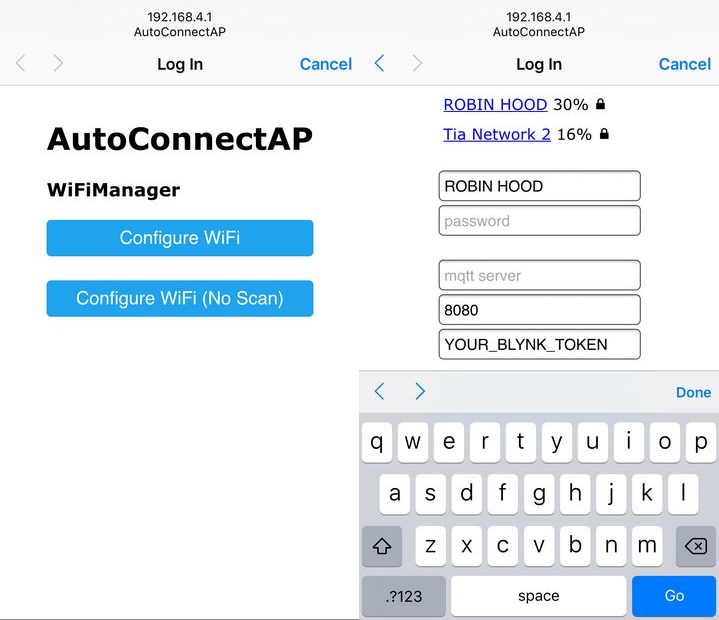
\includegraphics[scale=0.3]{images/wifi-access-point}
    \caption{Portal za odabir mreže (Izvor:~\cite{wifi-manager})}
\end{wrapfigure}

Ukoliko je dostupna mreža na koju se mikrokontroler povezao u prošlosti automatski se povezuje na nju.
U suprotnom mikrokontroler se ponaša kao pristupna točka (eng. \textit{access point}) i zahtjeva manualan odabir
bežične mreže i lozinke.
Pomoću drugog uređaja (npr.~\textit{smartphone}) potrebno je povezati se na mrežu imena \textit{ACCESS\_POINT\_NAME} s
lozinkom \textit{ACCESS\_POINT\_PASSWORD}, a potom se otvara portal kroz koji se konfigurira mreža na koju će se
mikrokontroler povezivati ubuduće.

